%\documentclass[dvipdfmx]{beamer}      % platex の場合
\documentclass[handout]{beamer}        % lualatex の場合
\usepackage{mySld}

\begin{document}
\title{基礎コンピュータ工学\\第3章 組み立て\\(パート2)}
\date{}

\begin{frame}
  \titlepage
  \centerline{\url{https://github.com/tctsigemura/TecTextBook}}
  \vfill
  \centerline{本スライドの入手:
    \raisebox{-7mm}{
\includegraphics[scale=0.3]{../Img/QRs3_2.png}}}
\end{frame}

%==============================================================================
%\begin{frame}
%  \frametitle
%  \tableofcontents
%\end{frame}

\section{組み立て}
%==============================================================================
\begin{frame}
  \frametitle{IC(1)}
  \vfill
  \centerline{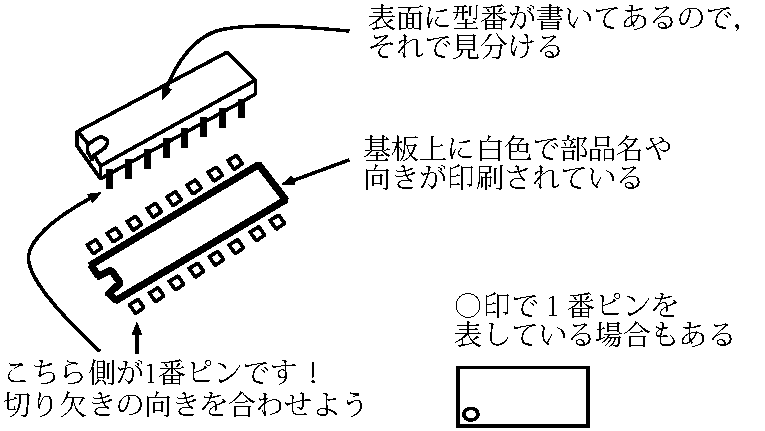
\includegraphics[scale=0.65]{../chap3/ic.pdf}}
  \vfill
  \centerline{\small\begin{tabular}{l|l|l}
    \hline
    \hline
    \multicolumn{1}{c|}{記号} &
    \multicolumn{1}{c|}{型番} &
    \multicolumn{1}{c}{説明} \\
    \hline
    U3 & K516       & 水晶発振 IC \\
    U6 & LM339      & 電圧比較 IC \\
  \end{tabular}}
\end{frame}

%==============================================================================
\begin{frame}
  \frametitle{IC(2)}
  \vfill
  \centerline{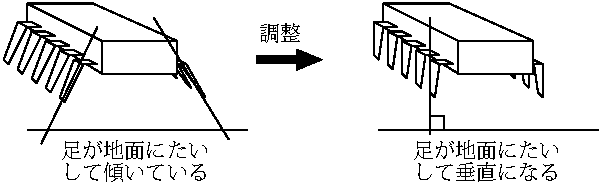
\includegraphics[scale=0.8]{../chap3/icnoasi.pdf}}
  \vfill
  \begin{itemize}
  \item ICには向きがあるので注意!!
  \item 足が基板に垂直になるように手直しする.(動画を参考に)
  \item 対角線上の二箇所を仮のハンダ付けする.\\
    → 浮き上がりは,まだ,修正できる.\\
    → 向きを間違っている場合は先生に頼む.
  \item 三つ以上の足をハンダ付けしたあとでは修正が難しい.
  \end{itemize}
\end{frame}

%==============================================================================
\begin{frame}
  \frametitle{集合抵抗器とラダー抵抗器}
  \begin{minipage}{0.45\columnwidth}
    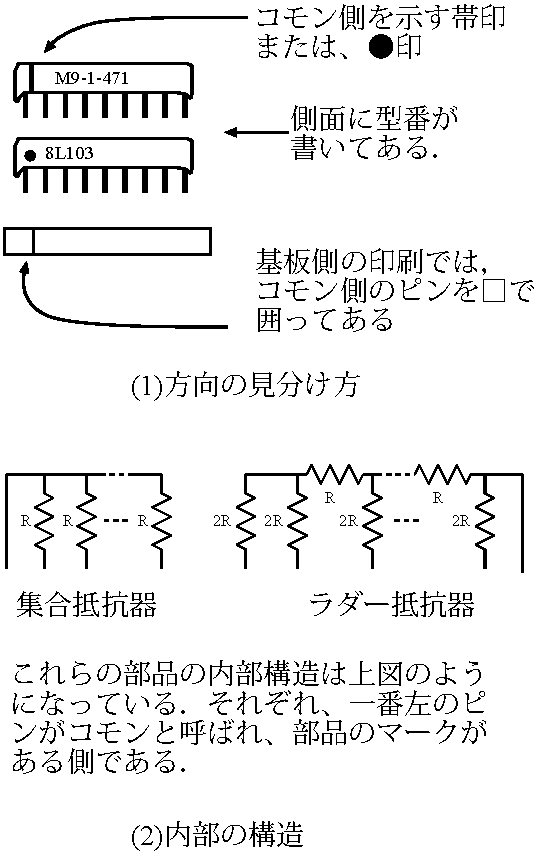
\includegraphics[scale=0.56]{../chap3/syuugou.pdf}
  \end{minipage}
  \begin{minipage}{0.54\columnwidth}
    \begin{center}
      {\footnotesize\begin{tabular}{l|l|l}
        \hline
        \hline
        \multicolumn{1}{c|}{記号} &
        \multicolumn{1}{c|}{型番} &
        \multicolumn{1}{c}{説明} \\
        \hline
        RA1,2 & M9-1-471   & 470Ω(8素子) \\
        &(L91S 471)&               \\
        RA3   & M9-1-391   & 390Ω(8素子) \\
        &(L91S 391)&               \\
        RA4   & M5-1-391   & 390Ω(4素子) \\
        &(L51S 391)&               \\
        RA5   & 8L103      & ラダー抵抗器  \\
      \end{tabular}}
    \end{center}
  \end{minipage}
\end{frame}

%==============================================================================
\begin{frame}
  \frametitle{フェライトビーズ}
  \centerline{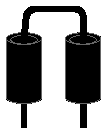
\includegraphics[scale=0.9]{../Tikz/bead.pdf}}
  \vfill
  \centerline{\small\begin{tabular}{l|l|l}
    \hline
    \hline
    \multicolumn{1}{c|}{記号} &
    \multicolumn{1}{c|}{型番} &
    \multicolumn{1}{c}{説明} \\
    \hline
    FB1,2 & なし & なし \\
  \end{tabular}}
  \vfill
  \begin{itemize}
    \item 向きはない.
    \item やけどに注意!!
  \end{itemize}
\end{frame}

%==============================================================================
\begin{frame}
  \frametitle{}
  \begin{minipage}{0.55\columnwidth}
    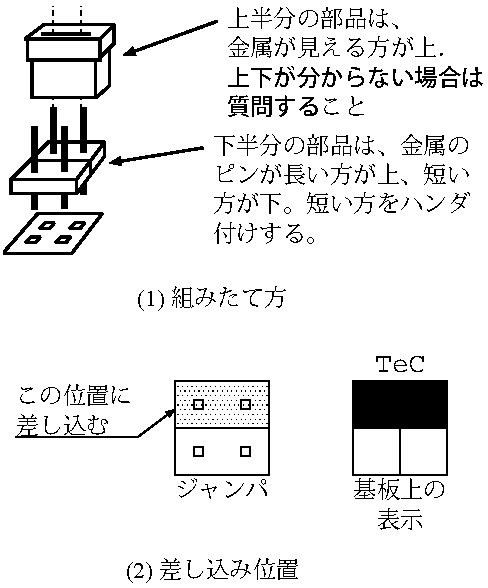
\includegraphics[scale=0.8]{../chap3/jp.pdf}
  \end{minipage}
  \begin{minipage}{0.44\columnwidth}
    \begin{center}
      {\small\begin{tabular}{l|l|l}
        \hline
        \hline
        \multicolumn{1}{c|}{記号} &
        \multicolumn{1}{c|}{型番} &
        \multicolumn{1}{c}{説明} \\
        \hline
        J1 & なし &  なし \\
        \end{tabular}}
    \end{center}
  \end{minipage}
\end{frame}

%==============================================================================
\begin{frame}
  \frametitle{圧電スピーカ}
  \centerline{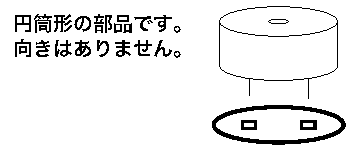
\includegraphics[scale=0.8]{../Tikz/buz.pdf}}
  \vfill
  \centerline{\small\begin{tabular}{l|l|l}
    \hline
    \hline
    \multicolumn{1}{c|}{記号} &
    \multicolumn{1}{c|}{型番} &
    \multicolumn{1}{c}{説明} \\
    \hline
    BZ1 & なし & 圧電スピーカ \\
  \end{tabular}}
\end{frame}

%==============================================================================
\begin{frame}
  \frametitle{電解コンデンサ}
  \centerline{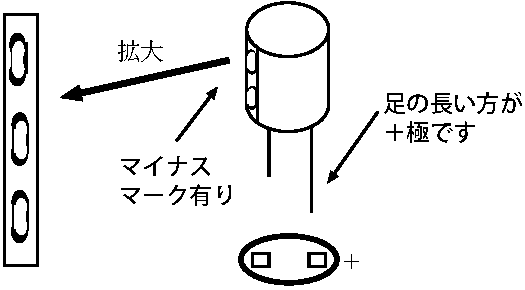
\includegraphics[scale=0.7]{../chap3/denkai.pdf}}
  \vfill
  \centerline{\small\begin{tabular}{l|l|l}
    \hline
    \hline
    \multicolumn{1}{c|}{記号} &
    \multicolumn{1}{c|}{型番} &
    \multicolumn{1}{c}{説明} \\
    \hline
    C0,C5,C7,C9,C16 & $ 25V 47 \mu F $ & $ 47 \mu F$ \\
    C11             & $ 10V 220 \mu F $ & $ 220 \mu F$ \\
  \end{tabular}}
  \vfill
  \begin{itemize}
  \item 向きがあるので注意!!
  \item 部品の浮き上がりに注意!!(やがて足が折れる)
  \end{itemize}
\end{frame}

%==============================================================================
%\begin{frame}
%  \frametitle{}
%\end{frame}

\end{document}
